\documentclass[tikz,border=4pt]{standalone}
\usepackage{tikz}
\begin{document}
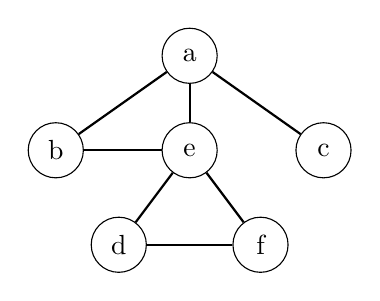
\begin{tikzpicture}[
  vertex/.style={circle,draw,minimum size=7mm,inner sep=0pt},
  edge/.style={line width=0.8pt}
]
\node[vertex] (a) at (0,2.4) {a};
\node[vertex] (b) at (-1.7,1.2) {b};
\node[vertex] (e) at (0,1.2) {e};
\node[vertex] (c) at (1.7,1.2) {c};
\node[vertex] (d) at (-0.9,0) {d};
\node[vertex] (f) at (0.9,0) {f};

\draw[edge] (a)--(b);
\draw[edge] (a)--(e);
\draw[edge] (a)--(c);
\draw[edge] (b)--(e);
\draw[edge] (e)--(d);
\draw[edge] (e)--(f);
\draw[edge] (d)--(f);
\end{tikzpicture}
\end{document}
